\chapter{The Rearrangement Number}

In contrast to the growth functions related cardinal characteristics this one is really easy to motivate, even for undergrads. It's known by the Riemann Rearrangement Theorem that any conditionally convergent (c.c.) series can be rearranged so it converges to any real, diverges by $\pm\infty$ or oscillates. Another way to state this theorem is as a property of $\sym$:
\begin{theorem}{}{}\textbf{(Riemann Rearrangement)}
    Given any c.c. series $\sum_n a_n$ and $\alpha,\beta\in\mbb{R}\cup\{\pm\infty\}$, there is some permutation $p\in\sym$ such that
    $$\limsup_m\sum_{n=0}^m a_{p(n)}=\alpha\quad\text{and}\quad\liminf_m\sum_{n=0}^ma_{p(n)}=\beta$$
\end{theorem}
One natural generalization one can think about is: how much smaller could we choose $\sym$? It turns out that we can define this in terms of cardinality as we will see, but it's far from trivial what this cardinal should be. We will prove this is a cardinal characteristic of the continuum, but it is still open if we can prove the equality with any well-known cardinal characteristic.

\section{Definitions}

\begin{definition}{}{}
    $\mf{rr}$ is the smallest cardinality of any family $C\subseteq\sym$ such that, for every c.c. series $\sum_n a_n$ of reals, there is some $p\in C$ for which $\sum_n a_{p(n)}$ no longer converges to the same limit.
\end{definition}

Analogously, if $\sum_n a_{p(n)}$ is required to converge, diverge to $\pm\infty$ or diverge by oscillation, then we have new cardinals $\mf{rr}_f$, $\mf{rr}_i$ and $\mf{rr}_o$, respectively.

We could also consider joints of those conditions, like $\mf{rr}_{fi}$ where $\sum_n a_{p(n)}$ either converges or diverges to $\pm\infty$.

Its easy to see that, if $C\subseteq\sym$ satisfies, for example, $\mf{rr}_i$, then it also satisfies $\mf{rr}_{fi}$, so $\mf{rr}_{fi}\leq\mf{rr}_i$, in general, we can make the Hasse Diagram in Figure \ref{fig:hasse-rearrangement}.

\begin{figure}[ht]
\centering
\begin{tikzcd}
	& {\mf{rr}_f} & {\mf{rr}_i} & {\mf{rr}_o} \\
	{} & {\mf{rr}_{fi}} & {\mf{rr}_{fo}} & {\mf{rr}_{io}} \\
	&& {\mf{rr}}
	\arrow[no head, from=1-2, to=2-2]
	\arrow[no head, from=1-2, to=2-3]
	\arrow[no head, from=1-3, to=2-2]
	\arrow[no head, from=1-3, to=2-4]
	\arrow[no head, from=1-4, to=2-3]
	\arrow[no head, from=1-4, to=2-4]
	\arrow[no head, from=2-2, to=3-3]
	\arrow[no head, from=2-3, to=3-3]
	\arrow[no head, from=2-4, to=3-3]
\end{tikzcd}
\caption{Hasse Diagram of the Rearrangement Numbers}
\label{fig:hasse-rearrangement}
\end{figure}

using this notation, $\mf{rr}$ would be $\mf{rr}_{fio}$, as expected.

\section{Padding with Zeros}

By Riemann's rearrangement $\mf{rr}\leq\lvert\sym\rvert=\mf{c}$, so, if $\mf{rr}$ is uncountable, then its a cardinal characteristic of the continuum.

Indeed, to prove that $\lvert\sym\rvert=\mf{c}$, note that $\sym\subseteq\omega^\omega$, therefore $\lvert\sym\rvert\leq\aleph_0^{\aleph_0}=2^{\aleph_0}$, so we will construct an injection $\varphi:[0,1]\to\sym$, s.t. for each real number $a=(0.d_0d_1d_2\dots)_2\in[0,1]$ we associate $\varphi(a)$ as the bijection in $\omega$ that swaps $2n$ with $2n+1$ if $d_n=1$, and does not swap them if $d_n=0$.

In this subsection we will prove its actually a cardinal characteristic and we will also explain an important technique about padding zeros.

\begin{theorem}{}{}\label{rr uncountable}
    $\mf{rr}$ is uncountable.
\end{theorem}

\begin{sketch}
    Let $C=\{p_n:n\in\omega\}$ be any countable subset of $\sym$ we will find a c.c. sequence that can't be corrupted by any of the permutations in $C$. To do this, we will start with any c.c. series, let's say $b_n=\frac{(-1)^n}{n}$ and we will pad a lot of zeroes between the terms and create a new sequence $a_n$ such that $\sum_n a_n=\sum_n a_{p_m(n)}$, $\forall m\in\omega$. We will do this defining a new function $\ell(n)$ such that $a_n=0$ if $n\notin\text{ran}(\ell)$, so, if in the summation we take only the non zero terms, we will have to prove that
    $$\sum_k a_{\ell(k)}=\sum_k a_{p_m(k)}$$
    then, to force $\ell(1),\ell(2),\dots$ to eventually appear in the same order as the $p_m(k)$'s, we need to preserve the relative order of the terms $\ell(n)$ for almost all $n$, for example
    $$p_m^{-1}(\ell(m))<p_m^{-1}(\ell(m+1))<p_m^{-1}(\ell(m+2))<\dots$$
    so, we want to avoid that $p_m^{-1}(\ell(k))>p_m^{-1}(\ell(k+1))$, for some $m\leq k$. Then, to reach a contradiction, we could say that $\ell(k+1)\neq p_m(j)$, for any $p_m^{-1}(\ell(k))>j$ and $m\leq k$.
\end{sketch}

\begin{proof}
    Assume by contradiction that there is a $C=\{p_n:n\in\omega\}\subseteq\sym$, Let $b_n:=\frac{(-1)^n}{n}$ (indeed, we can take any term of a c.c. series). Lets define $\ell:\omega\to\omega$ a fast growing function that will indicate the new position of $b_k$ and will add a lot of $0$'s between the $b_k$'s, i.e.
    $$a_n:=\begin{cases}
        b_k,\, n=\ell(k)\\
        0,\, \text{otherwise}
    \end{cases}$$
    So, define $\ell(0)=0$ and, given $\ell(k)$ defined, let $\ell(k+1)>\ell(k)$ such that $\ell(k+1)\neq p_m(j)$, $j\leq p_m^{-1}(\ell(k))$, $m\leq k$ (which exists, since there are finite terms $p_m(j)$ of that form).

    Now, we claim that $\forall m\geq k$, $p_m^{-1}(\ell(k))<p_m^{-1}(\ell(k+1))$, in fact, if there was a $m\leq k$ s.t. $p_m^{-1}(\ell(k))>p_m^{-1}(\ell(k+1))$, then, for $j=p_m^{-1}(\ell(k+1))$, by hypothesis
    $$\ell(k+1)\neq p_m\rp{p_m^{-1}(\ell(k+1))}=\ell(k+1)$$
    a contradiction. So, we finally have that, $\forall m\in\omega$
    $$p_m^{-1}(\ell(m))<p_m^{-1}(\ell(m+1))<p_m^{-1}(\ell(m+2))<\dots$$
    so, $p_m^{-1}$ preserves the relative order of $b_k$'s, except for possibly the first $m$ terms, so, its clear that
    $$\sum_n a_n=\sum_n a_{p_m(n)},\,\forall m\in\omega$$
\end{proof}

\section{Mixing Permutations}
In this subsection we will prove some equalities on the variants of the rearrangement number by explaining an important technique called The Mix Lemma.

\begin{lemma}{}{}\label{mix}\textbf{(The Mix Lemma)}
    For all $p,q\in\sym$, there is a $g\in\sym$ such that:
    \begin{itemize}
        \item $g[n]=p[n]$ for infinitely many $n$'s;
        \item $g[n]=q[n]$ for infinitely many $n$'s
    \end{itemize}
\end{lemma}

To prove The Mix Lemma we will first prove the following lemma

\begin{lemma}{}{}\label{pre-mix}
    For any $p\in\sym$, if $h:n\to\omega$ is injective, then there exists $h\subseteq h':M\to\omega$, with $M>n$, such that $\text{Im}(h')=p[M]$.
\end{lemma}

\begin{proof}
    Since $p$ is a bijection, there are $m_0,m_1,\dots,m_{n-1}$ such that $p(m_i)=h(i)$, so, if we choose $M=\max\{m_0,m_1,\dots,m_{n-1}\}+2>n$, then $h[n]=\text{Im}(h)\subseteq p[M]$ and $h'=p\lvert_M$ do the job.
\end{proof}

Now, let's prove the mix lemma

\begin{proof}\textbf{(The Mix Lemma.)} Let $g_0=\emptyset$. If $g_{2k-1}:n_{2k-1}\to\omega$ was already defined, by the previous lemma there exists a $g_{2k}:n_{2k}\to\omega$ extending $g_{2k-1}$ s.t. $\text{Im}(g_{2k})=p[n_{2k}]$. Analogously, if $g_{2k}$ was already defined, let $g_{2k+1}:n_{2k+1}\to\omega$ extending $g_{2k}$ s.t. $\text{Im}(g_{2k+1})=q[n_{2k+1}]$.

Since $\{g_n:n\in\omega\}$ is a family of compatible functions, then $g:=\bigcup_{n\in\omega}g_n$ is well defined. To show $g\in\sym$, note first that, since by the previous lemma $M>n$, then $n_k>n_m$, $\forall k>m$, therefore $\text{dom}(g)=\omega$ and, since each $g_k$ is injective, $g$ is also. Now, for any $k\in\omega$, there is a $k'\in\omega$ s.t. $p(k')=k$ and, since $g$ agrees with $p$ for infinitely many $n$'s, then $k$ is eventually in the image of $g$. Therefore we have that $g\in\sym$.
\end{proof}

Now, lets narrow down how much rearrangement numbers are there

\begin{theorem}{}{}\label{rr=rr_ifo}
    $$\mf{rr}=\mf{rr}_{fo}=\mf{rr}_{io}=\mf{rr}_o$$
\end{theorem}

\begin{proof}
    Since $\mf{rr}_o\geq\mf{rr}_{fo},\mf{rr}_{io}\geq\mf{rr}$, its sufficient to show that $\mf{rr}\geq\mf{rr}_o$.

    Let $C\subseteq\sym$ be as in the definition of $\mf{rr}$, by The Mix Lemma \ref{mix}, for each $p\in C$ there is a $g_p\in\sym$ s.t. $g_p$ agrees with $p$ and $q=\text{id}$ for infinitely many $n$'s. Define
    $$C':=C\cup\{g_p:p\in C\}$$
    By the previous theorem, $\lvert C\rvert>\aleph_0$, so $\lvert C'\rvert=\lvert C\rvert=\mf{rr}$. We will show that $C'$ satisfies $\mf{rr}_o$.

    Let $\sum_n a_n$ be c.c., we know that there exists a $p\in C$ that corrupts the series. If $\sum_n a_{p(n)}$ diverges by oscillation, we are done, otherwise, if it diverges for infinity, or converges to a different number, then $\sum_n a_{g_p(n)}$ has a subsequence going to infinity or this new sum, and another going to the original sum, so it diverges by oscillation.
\end{proof}
The previous theorem narrows down the number of rearrangement cardinals (Figure \ref{fig:rearrangement-narrowed})

\begin{figure}[ht]
\centering
\begin{tikzcd}
	{\mf{rr}_f} && {\mf{rr}_i} \\
	& {\mf{rr}_{fi}} \\
	& {\mf{rr}}
	\arrow[no head, from=1-1, to=2-2]
	\arrow[no head, from=1-3, to=2-2]
	\arrow[no head, from=2-2, to=3-2]
\end{tikzcd}
\caption{Narrowed Hasse Diagram}
\label{fig:rearrangement-narrowed}
\end{figure}

\section{Measure and Random Signs}

In this subsection we relate the rearrangement number with the covering number for measure. In order to relate them we will need a consequence of Kolmogorov's Two Series Theorem, whose proof depends on the following inequality also due to Kolmogorov:

\begin{lemma}{}{}
    \textbf{(Kolmogorov's Inequality)} Let $X_1,X_2,\dots,X_n$ be independent random variables with $\mbb{E}[X_k]=0$ and $\text{var}(X_k)<\infty$ for $k=1,\dots,n$. Then, $\forall\varepsilon>0$ we have that:
    $$\mbb{P}\rp{\max_{1\leq k\leq n}\lvert S_k\rvert\geq\varepsilon}\leq\frac{\text{var}(S_n)}{\varepsilon^2}=\frac1{\varepsilon^2}\sum_{k=1}^n\text{var}(X_k)$$
    where $S_k=X_1+X_2+\dots+X_k$.
\end{lemma}

\begin{proof}
    Let $E=\left\{\max_{1\leq k\leq n}\lvert S_k\rvert\geq\varepsilon\right\}$ and consider the events
    $$E_k=\left\{\lvert S_1\rvert<\varepsilon,\lvert S_2\rvert<\varepsilon,\dots,\lvert S_{k-1}\rvert<\varepsilon,\lvert S_k\rvert\geq\varepsilon\right\}$$
    Clearly $E_k$ are disjoint and $E=\bigcup_{k=1}^nE_k$, therefore
    \begin{equation}\label{p(e)}
        \mbb{P}(E)=\sum_{k=1}^n\mbb{P}(E_k)
    \end{equation}
    Furthermore, since $\mbb{E}[X_k]=0$, $k=1\dots,n$, then $\mbb{E}[S_n]=0$. And, since $S_n^2$ is always greater or equal than $0$, then $\mbb{E}[S_n^2]\geq\mbb{E}[S_n^2\cdot I_A]$ for any event $A$, consequently:
    \begin{equation}\label{var(S_n)}
        \text{var}(S_n)=\mbb{E}[S_n^2]\geq\mbb{E}[S_n^2\cdot\boldsymbol{1}_E]=\sum_{k=1}^n\mbb{E}[S_n^2\cdot\boldsymbol{1}_{E_k}]
    \end{equation}
    Now, note that
    $$S_n^2=(S_n+(S_k-S_n))^2=S_k^2+2S_k(S_n-S_k)+(S_n-S_k)^2$$
    therefore, multiplying by $\boldsymbol{1}_{E_k}$ and taking the expected value at both sides
    $$\mbb{E}[S_n^2\cdot\boldsymbol{1}_{E_k}]=\mbb{E}[S_k^2\cdot\boldsymbol{1}_{E_k}]+2\mbb{E}[S_k(S_n-S_k)\cdot\boldsymbol{1}_{E_k}]+\mbb{E}[(S_n-S_k)^2\cdot\boldsymbol{1}_{E_k}]$$
    but $S_k\cdot\boldsymbol{1}_{E_k}=(X_1+\dots X_k)\cdot\boldsymbol{1}_{E_k}$ and $S_n-S_k=X_n+X_{n-1}+\dots+X_{k+1}$ and, since $X_k$ are independent, $S_k\cdot\boldsymbol{1}_{E_k}$ and $S_n-S_k$ are also independent, then
    $$\mbb{E}[S_k(S_n-S_k)\cdot\boldsymbol{1}_{E_k}]=\mbb{E}[S_k\cdot\boldsymbol{1}_{E_k}]\cdot\cancelto0{\mbb{E}[S_n-S_k]}=0$$
    so we can conclude that
    \begin{equation}\label{E(S_n2 1_E)}
        \mbb{E}[S_n^2\cdot\boldsymbol{1}_{E_k}]=\mbb{E}[S_k^2\cdot\boldsymbol{1}_{E_k}]+\mbb{E}[(S_n-S_k)^2\cdot\boldsymbol{1}_{E_k}]\geq\mbb{E}[S_k^2\cdot\boldsymbol{1}_{E_k}]
    \end{equation}
    now, substituting \ref{E(S_n2 1_E)} in \ref{var(S_n)}, we conclude that
    $$\text{var}(S_n)\geq\sum_{k=1}^n\mbb{E}[S_n^2\cdot\boldsymbol{1}_{E_k}]\geq\sum_{k=1}^n\mbb{E}[S_k^2\cdot\boldsymbol{1}_{E_k}]$$
    and, by definition, $\lvert S_k(\omega)\rvert\geq\varepsilon$ whenever $\boldsymbol{1}_{E_k}(\omega)$, therefore $\lvert S_k^2(\omega)\rvert\geq\varepsilon^2$ and, by \ref{p(e)}, we have that
    $$\text{var}(S_n)\geq\sum_{k=1}^n\mbb{E}[\varepsilon^2\cdot\boldsymbol{1}_{E_k}]=\varepsilon^2\sum_{k=1}^n\mbb{P}(E_k)=\varepsilon^2\mbb{P}(E)$$
\end{proof}

\begin{theorem}{}{}
    \textbf{(Kolmogorov's Two Series)}. Let $(X_n)_{n\geq0}$ be independent random variables. If $\sum_n\mbb{E}[X_n]$ and $\sum_n\text{var}(X_n)$ both converges, then $\sum_n X_n$ converges almost surely.
\end{theorem}

\begin{proof}
    Note first that, if we define $Y_k=X_k-\mbb{E}[X_k]$, then $Y_k$ are also independent, $\mbb{E}[Y_n]=0$ and $\text{var}(Y_n)=\text{var}(X_n)$. Now, since
    $$\sum_n X_n=\sum_n(Y_n+\mbb{E}[X_n])=\sum_n Y_n+\sum_n\mbb{E}[X_n]$$
    and, by hypothesis, $\sum_n\mbb{E}[X_n]$ converges, then $\sum_n X_n$ converges iff $\sum_n Y_n$ converges, then we can assume WLOG that $\mbb{E}[X_n]=0$.

    We will show that, if $S_k=\sum_{i=1}^kX_k$, then $\mbb{P}(S_k\text{ converges})=1$ or, equivalently, that $S_k$ is almost surely Cauchy. In order to do that, note that
    $$\max_{m,n\geq N}\lvert S_n-S_m\rvert\leq\max_{n\geq N}\lvert S_n-S_N\rvert+\max_{m\geq N}\lvert S_n-S_M\rvert\leq2\max_{n\geq N}\lvert S_n-S_N\rvert$$
    then, by Kolmogorov's Inequality
    \begin{equation}\label{kolmogorov S_n}
        \mbb{P}\rp{\max_{m,n\geq N}\lvert S_n-S_m\rvert>\varepsilon}\leq\mbb{P}\rp{\max_{n\geq N}\lvert S_n-S_N\rvert>\frac\varepsilon2}\leq\frac4{\varepsilon^2}\sum_{n=N+1}^n\text{var}(S_n)
    \end{equation}
    Now, note that, $S_n$ is not Cauchy if, there is a $\varepsilon>0$ rational such that, for all $N\in\omega$, there are $n,m\geq N$ with $\lvert S_n-S_m\rvert>\varepsilon$. Then, for $S_n$ to be almost surely Cauchy it's sufficient that
    $$\mbb{P}\rp{\bigcup_{\varepsilon\in\mbb{Q}}\bigcap_{N\in\omega}\bigcup_{n,m\geq N}\left\{\lvert S_n-S_m\rvert>\varepsilon\right\}}\leq\sum_{\varepsilon
    \in\mbb{Q}}\;\mbb{P}\rp{\bigcap_{N\in\omega}\bigcup_{n,m\geq N}\left\{\lvert S_n-S_m\rvert>\varepsilon\right\}}=0$$
    or that $\mbb{P}\rp{\bigcap_{N\in\omega}\bigcup_{n,m\geq N}\left\{\lvert S_n-S_m\rvert>\varepsilon\right\}}=0$. But, if $E_N=\bigcup_{n,m\geq N}\left\{\lvert S_n-S_m\rvert>\varepsilon\right\}$, note that $E_n\supseteq E_{n+1}$, $\forall n\in\omega$, then, we have
    $$\mbb{P}\rp{\bigcap_{N\in\omega}E_N}=\lim_{N\to\infty}\mbb{P}(E_N)$$
    and, since $E_N=\max_{m,n\geq N}\lvert S_n-S_m\rvert>\varepsilon$, by \ref{kolmogorov S_n} we have that
    $$\lim_{N\to\infty}\mbb{P}(E_N)\leq\lim_{N\to\infty}\frac4{\varepsilon^2}\sum_{n=N+1}^n\text{var}(S_n)=0$$
    where the summation is $0$ because $\sum_n\text{var}(S_n)$ converges. Then $S_n$ is almost surely Cauchy.
\end{proof}

Using Kolmogorov's Theorem we can prove the following Lemma due to Rademacher

\textcolor{laser_eyes}{Como usaremos somente $c_n=\frac1n$ na prova do teorema 2.5., e sabemos que a harmônica se relaciona com a densidade assintótica por meio do ln, talvez seja possível pular esse teorema}

\begin{theorem}{}{}
    \textbf{(Rademacher).} Let $(c_n)_{n\geq0}$ be any sequence of reals. And let
    $$A:=\left\{s\in2^\omega:\sum_n(-1)^{s(n)}c_n\text{ converges}\right\}$$
    Then $\lambda(A)=1$ if $\sum_nc_n^2$ converges.
\end{theorem}

\begin{proof}
    We will consider $X_n=(-1)^{s(n)}c_n$, where $s_n$ is $0$ and $1$ with probability $\frac12$. Now
    $$\mbb{E}[X_n]=\mbb{E}[(-1)^{s(n)}c_n]=c_n\rp{1\cdot\frac12+(-1)\cdot\frac12}=0$$
    Therefore $\sum_n\mbb{E}[X_n]$ converges. Now $\text{var}(Y_n)=\mbb{E}[Y_n^2]-\mbb{E}[Y_n]^2$ and, since we have that
    $$\mbb{E}[Y_n^2]=c_n^2\rp{1\cdot\frac12+1\cdot\frac12}=c_n^2$$
    then the second series became $\sum_nc_n^2$, which converges by assumption. And, by Kolmogorv's Two Series Theorem, $\lambda(A)=1$.
\end{proof}
With the previous theorem we can now give an inequality between $\text{cov}(\mc{N})$ and $\mf{rr}$.

\begin{theorem}{}{}
    $\text{cov}(\mc{N})\leq\mf{rr}$
\end{theorem}

\textcolor{laser_eyes}{Aqui estamos usando que $\text{cov}(\mc{N})$ é o mesmo se $\mc{N}$ for escolhido em $\mbb{R}$ ou no Espaço de Cantor $2^\omega$.}

\begin{proof}
    Since $\sum_n\frac1{n^2}$ converges absolutely, for any $p\in\sym$, since $\sum_n\frac1{p(n)^2}$ is just a rearrangement, then it also converges. Now, by Rademacher's Theorem, for $c_n=\frac1{p(n)}$, the set
    $$A_p:=\left\{s\in2^\omega:\sum_n(-1)^{s(n)}/p(n)\text{ diverges}\right\}$$
    has measure zero. And, since $s\mapsto s\circ p$ is measure preserving in the Cantor Space $2^\omega$ \textcolor{laser_eyes}{(Por que?)}, then $B_p=p[A_p]$ also has measure zero.

    Now, let $C\subseteq\sym$ be s.t. $\lvert C\rvert<\text{cov}(\mc{N})$. By definition of $\text{cov}(\mc{N})$, we have that $\{B_p\}_{p\in C}$ cannot cover $2^\omega$, then there is some $s\in2^\omega$ such that $\sum_n(-1)^{s(p(n))}/p(n)$ converges $\forall p\in C$. That is, the rearrangement of $\sum_n(-1)^{s(n)}/n$ will not diverge to $\pm\infty$ or oscillate.

    Therefore, this proves that $\text{cov}(\mc{N})\leq\mf{rr}_{io}=\mf{rr}$.
\end{proof}

\section{Topology and Some Inequalities}

In this subsection we will continue to present some inequalities between the rearrangement numbers and other well known cardinal characteristic, so we can try, for example, to see where the rearrangement numbers are in the Cichóns Diagram.

For the first inequality, we will need the following lemmas

\begin{lemma}{}{}\label{comeager-lemma}
    If $Y\subseteq X$ and $X$ is meager, then $Y$ is also meager.
\end{lemma}

\begin{proof}
    Since $X$ is meager, $X=\bigcup_{n\in\omega}X_n$, where each $X_i$ is nowhere dense, i.e., $\text{int}\rp{\ol{X_i}}=\emptyset$, $\forall i\in\omega$. Now, since $Y\subseteq X$, we have that
    \begin{equation}
        Y=Y\cap X=\bigcup_{n\in\omega}Y\cap X_n\tag{$*$}
    \end{equation}
    but $Y\cap X_i\subseteq X_i$, which implies $\ol{Y\cap X_i}\subseteq\ol{X_i}$, then $\text{int}\rp{\ol{Y\cap X_i}}\subseteq\text{int}\rp{\ol{X_i}}=\emptyset$, i.e., $Y\cap X_i$ are nowhere dense, therefore by $(*)$ $Y$ is also meager.
\end{proof}

\begin{lemma}{}{}
    The subspace $\sym$ of $\omega^\omega$ of all permutations of $\omega$ is homeomorphic to $\omega^\omega$
\end{lemma}

\begin{proof}
    \textcolor{laser_eyes}{Uma possível demonstração usa o Teorema de Alexandrov-Uryhson, cujos pré-requisitos estão far beyond what I know. Outra possível demonstração é a construção direta do homeomorfismo como eles fazem no artigo do número de rearranjo, mas não é muito intuitiva.}
\end{proof}

\begin{corollary}{}{}
    Let $\mc{M}_X$ be the set of meager sets in the space $X$. If $X\cong Y$, then
    $$\text{non}(\mc{M}_X)=\text{non}(\mc{M}_Y)$$
\end{corollary}

\begin{proof}
    By symmetry, it's sufficient to show that, if $f:X\cong Y$, then $A$ is meager in $X$ implies $f(A)$ is meager in $Y$. It's a classical result in topology that, if $f$ is a homeomorphism, then it commutes with $\text{cl}$ and $\text{int}$. Therefore, if $A=\bigcup_{n\in\omega}A_n$, with $\text{int}\rp{\ol{A_n}}=\emptyset$, then
    $$f(A)=f\rp{\bigcup_{n\in\omega}A_n}=\bigcup_{n\in\omega}f(A_n)$$
    with $\text{int}\rp{\ol{f(A_n)}}=f\rp{\text{int}\rp{\ol{A}}}=\emptyset$, i.e., $f(A)$ is also meager.
\end{proof}

\begin{theorem}{}{}\label{rr<=non(M)}
    $$\mf{rr}\leq\textbf{non}(\mc{M})$$
\end{theorem}

\begin{proof}
    Its sufficient to prove that any non-meager set $C\subseteq\sym$ has, given some series, a permutation that corrupts it. Given a c.c. series $\sum_n a_n$ of reals, consider
    $$X(a_n):=\left\{p\in\sym:\sum_n a_{p(n)}\neq\sum_n a_n\right\}$$
    we need to show that $C\cap X(a_n)\neq\emptyset$, then, its sufficient to show that $X(a_n)$ is comeager, since, if it was empty, then $C\subseteq X(a_n)^c$, but, by Lemma \ref{comeager-lemma}, $C$ would also be meager.

    To show $X(a_n)$ is comeager, its sufficient to prove the stronger claim that
    $$Y(a_n):=\left\{p\in\sym:\sum_n a_{p(n)}=\infty\right\}$$
    is the intersection of countable many dense open sets, i.e. $Y=\bigcap_{n\in\omega}D_n$ with $D_n$ open and denses.
    
    In fact, first of all, since $D_n$ is open, $D_n^c$ is closed, then, if $\text{int}(\ol{D_n^c})=\text{int}(D_n^c)\neq\emptyset$, there would be an open $U\subseteq D_n^c$, so $U\cap D_n=\emptyset$, contradicting that $D_n$ is dense, therefore $D_n$ is nowhere dense for all $n\in\omega$. Now, since $Y^c=\bigcup_{n\in\omega}D_n^c$, $Y^c$ is meager and, since $Y(a_n)\subseteq X(a_n)$, then $X(a_n)^c\subseteq Y(a_n)^c$, so, by Lemma \ref{comeager-lemma}, $X(a_n)^c$ would be meager too.

    So, since we have that
    $$Y(a_n)=\bigcap_{k\in\omega}\bigcup_{m\geq k}\left\{p\in\sym:\sum_{n=0}^m a_{p(n)}\geq k\right\}$$
    its sufficient to prove that
    $$D_k:=\bigcup_{m\geq k}\left\{p\in\sym:\sum_{n=0}^m a_{p(n)}\geq k\right\}$$
    is dense and open. If $p\in D_k$, $\sum_{n=0}^m a_{p(n)}\geq k$ for some $m\geq k$. Then, given any $q\in\mc{N}(p\restriction_{m+1})$ extending $p$ until $m$, we have that
    $$\sum_{n=0}^m a_{q(n)}=\sum_{n=0}^m a_{p(n)}\geq k$$
    So $\mc{N}(p\restriction_{m+1})\subseteq D_k$, then its open. Now, we will prove its dense, i.e., for all $p\in\omega^{<\omega}$, we have $D_k\cap \mc{N}(p)\neq\emptyset$. Given $p\in\omega^{<\omega}$, extend it with positive terms to $p'$ with domain $\geq k$ such that $\sum_{n=0}^m a_{p'(n)}\geq k$, which exists, since $\sum_{n=0}^m a_n^+=\infty$.
\end{proof}

Its hard to see how to change the argument so that $\sum_n a_{p(n)}$ could converge or diverge to $\pm\infty$. In fact, you can't, this is not a defect of the argument, these large rearrangement numbers can consistently be larger than $\textbf{non}(\mc{M})$.

For the sake of the argument we will now prove the following inequality, which will be superseded by a stronger one in the next subsection.

\begin{theorem}{}{}
    $$\mf{rr}_{fi}\geq\textbf{cov}(\mc{M})$$
\end{theorem}

\begin{proof}
    Given $p\in\sym$ consider the set
    \begin{align*}
        A_p & := \left\{g\in\sym:g[M]=p[M]\text{ for infinitely many }M\right\}\\
        & = \bigcap_{m\in\omega}\bigcup_{n\geq m}\left\{g\in\sym:g[n]=p[n]\right\}
    \end{align*}
    as we saw in \ref{rr<=non(M)}, to show $A_p$ is comeager, its sufficient to show that
    $$U_m:=\bigcup_{n\geq m}\{g\in\sym:g[n]=p[n]\}=\bigcup_{n\geq m}B_n$$
    is open and dense. In fact, given $g\in U_m$, then $g\in B_k$ for some $k\geq m$, so $\mc{N}(g(0),\dots,g(k))\subseteq U_m$, then it's open. Now, given $p\in\sym$, $p$ is injective, so, by The Mix Lemma \ref{mix}, it can be extended to $p'\in\sym$ s.t. $p[n]=p'[n]$ for infinitely many $n\in\omega$, so $p'\in \mc{N}(p(0),\dots,p(k))\cap U_m$, for any $k\in\omega$, so it's dense.

    Now, suppose toward a contradiction that $\mf{rr}_{fi}<\textbf{cov}(\mc{M})$ and let $C$ witness this. Assume WLOG that $\text{id}\in C$. Since $\bigcap_{p\in C}A_p$ is the intersection of fewer than $\textbf{cov}(\mc{M})$ comeager sets, it's nonempty, so let $g$ be a member of it.

    Then, for any c.c. series $\sum_n a_n$, let $p\in C$ be such that $\sum_n a_{p(n)}$ converges to a different number or diverges to infinity. Since $g\in A_p$, $g[M]=p[M]$ for infinitely many $M$, and also $g[M]=M$ for infinitely many, since $\text{id}\in C$. As a result, the same argument as in \ref{rr=rr_ifo} shows that $\sum_n a_{g(n)}$ diverges by oscillation, so $\{g\}$ witnesses that $\mf{rr}_o=1$, a contradiction, since it's uncountable.
\end{proof}

\section{Advanced padding}

The key idea in the padding method was to spread out the nonzero terms in a series so far that the permutations under consideration do not change their relative order up to finitely many exceptions. Now we will introduce a cardinal characteristic intended to capture this idea.

\begin{definition}{}{} Let $A\subseteq\omega$
    \begin{itemize}
        \item $A$ is preserved by $p\in\sym$ if $p$ doesn't change the relative order of members of $A$, except for finitely many elements. If $A$ is not preserved by $p$ we say it's jumbled by $p$.
        \item A conserving family is a family of permutations such that there is an infinite set $A$ that is preserved by every $p$ in the family.
        \item The jumbling number $\mf{j}$ is the greatest cardinality of a conserving family.
    \end{itemize}
\end{definition}
Note that, if $S=\{q_n:n\in\omega\}\subseteq\sym$, let $C=\{p_m=q_m^{-1}:m\in\omega\}$, then, by doing the construction of the fast growing function $\ell:\omega\to\omega$ as in \ref{rr uncountable}, we guarantee that $p_m(\ell(m))<p_m(\ell(m+1))<\dots$, which means $A=\{\ell(n):n\in\omega\}$ is not jumbled by any $p\in C$, then, since $\aleph_0<\mf{j}\leq\lvert\sym\rvert=\mf{c}$, it's a cardinal characteristic of the continuum. This proof is not necessary, since Theorem \ref{j<=b} will guarantee that (but the argument is way harder. way more powerful, tho).

Roughly, $\mf{j}$ is defined to be the largest cardinal for which the argument in Theorem \ref{rr uncountable} remains valid. Just consider that for any fast growing such function $\ell$ we can associate the set $A=\{\ell(1),\ell(2),\dots\}$ and vice-versa. We will see how to use this in the proof of the next Theorem.

\begin{theorem}{}{}
    $$\mf{j}\leq\mf{rr}$$
\end{theorem}

\begin{proof}
    The idea is to use the same translation as in the proof that $\mf{j}$ is uncountable. Let $C\subseteq\sym$, with $\lvert C\rvert<\mf{j}$. We shall find a c.c. series that is not corrupted by $C$. Let $\sum_n b_n$ be any c.c. series and, since $\lvert C\rvert<\mf{j}$ let $A\subseteq\omega$ be the set that is not jumbled by \textit{the inverses of all permutations} in $C$. Then, using $A$ as the growing function, let
    $$a_n:=\begin{cases}
        b_k,\text{ if $n$ is the $k^{\text{th}}$ element of $A$}\\
        0,\text{ if $n\notin A$}
    \end{cases}$$
    If $p\in C$, then $A$ is preserved by $p^{-1}$, then the order of almost all nonzero terms of $\sum_n a_n$ and $\sum_n a_{p(n)}$ are the same, therefore $C$ does not corrupt $\sum_n a_n$.
\end{proof}

In order to bound $\mf{rr}$ with a well known cardinal characteristic, we will prove the following theorem

\begin{theorem}{}{}\label{j<=b}
    $\mf{j}\leq\mf{b}$, therefore, $\mf{b}\leq\mf{rr}$.
\end{theorem}

\begin{sketch}
    To prove $\mf{b}\leq\mf{j}$, we will take $C\subseteq\sym$ s.t. $\lvert C\rvert<\mf{b}$ and prove it cannot be a jumbling family. Since $\lvert C\rvert<\mf{b}$, we need to associate for each $p\in C$ a function $f_p:\omega\to\omega$ so we could have a function $g:\omega\to\omega$ that dominates $f_p$ for all permutations $p\in C$ and, using $g$, we will define a set $A\subseteq\omega$ that is not jumbled by $C$.

    Fixing $p\in C$, we want to define $f_p$ such that, for some $g\geq^* f_p$ and $A$ we will have, $p$ will preserve the order of most elements in $A$. Let's then define $f_p$ as an \textit{Stabilization Point}, i.e, $f_p(n)$ is s.t. from this point on, every number will have the image over $p$ greater than $p(1),p(2),\dots,p(n)$.

    As Figure \ref{fig:p-arrows} shows, given $1,2,3,\dots,n$, and labeling them $b_1,b_2,\dots,b_n$ such that $p(b_1)<p(b_2)<\dots<p(b_n)$ (points represented in purple), we know that for each number between the images of $1,2,\dots,n$ there will be some number $y_i$ that will go there (numbers in blue), then, if we run out all of them, any other number after those ones will necessarily be greater than the images of $1,2,\dots,n$ over $p$, then we just need to choose $f_p(n)$ (in red) far enough so he can surpass all these finite elements.

    Then, if we define $a_0\in\omega$ and $a_{n+1}\in\omega$ such that $a_{n+1}>g(a_n)$, it's easy to see that $A=\{a_i\}_{i\in\omega}$ is preserved by $C$.
\end{sketch}

\tikzset{every picture/.style={line width=0.75pt}} %set default line width to 0.75pt 

\begin{figure}[ht]
    \centering
    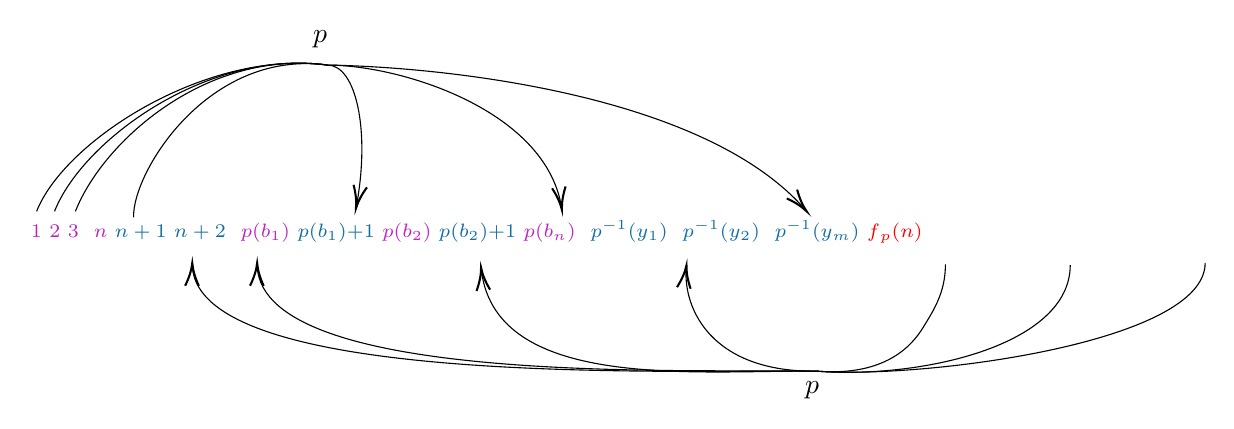
\begin{tikzpicture}[x=0.75pt,y=0.75pt,yscale=-1,xscale=1]
    %uncomment if require: \path (0,300); %set diagram left start at 0, and has height of 300
    
    %Curve Lines [id:da869685567152708] 
    \draw    (45,149.62) .. controls (58.66,115.11) and (127.68,71.25) .. (185.2,79.16) ;
    %Curve Lines [id:da45348245378320906] 
    \draw    (53.63,149.62) .. controls (67.29,115.11) and (127.68,71.25) .. (185.2,79.16) ;
    %Curve Lines [id:da15163922233603622] 
    \draw    (63.69,149.62) .. controls (77.35,115.11) and (127.68,71.25) .. (185.2,79.16) ;
    %Curve Lines [id:da4266797108919014] 
    \draw    (185.2,79.16) .. controls (198.66,79.16) and (205.84,109.86) .. (199.18,146.51) ;
    \draw [shift={(198.86,148.19)}, rotate = 280.89] [color={rgb, 255:red, 0; green, 0; blue, 0 }  ][line width=0.75]    (10.93,-3.29) .. controls (6.95,-1.4) and (3.31,-0.3) .. (0,0) .. controls (3.31,0.3) and (6.95,1.4) .. (10.93,3.29)   ;
    %Curve Lines [id:da09212583179865697] 
    \draw    (185.2,79.16) .. controls (220.79,79.16) and (290.21,101.01) .. (297.87,147.49) ;
    \draw [shift={(298.09,148.91)}, rotate = 262.23] [color={rgb, 255:red, 0; green, 0; blue, 0 }  ][line width=0.75]    (10.93,-3.29) .. controls (6.95,-1.4) and (3.31,-0.3) .. (0,0) .. controls (3.31,0.3) and (6.95,1.4) .. (10.93,3.29)   ;
    %Curve Lines [id:da05325802271682478] 
    \draw    (185.2,79.16) .. controls (236.71,79.88) and (365.81,91.98) .. (415.26,148.76) ;
    \draw [shift={(416,149.62)}, rotate = 229.64] [color={rgb, 255:red, 0; green, 0; blue, 0 }  ][line width=0.75]    (10.93,-3.29) .. controls (6.95,-1.4) and (3.31,-0.3) .. (0,0) .. controls (3.31,0.3) and (6.95,1.4) .. (10.93,3.29)   ;
    %Curve Lines [id:da5942864735244722] 
    \draw    (91.73,152.5) .. controls (91.02,130.93) and (127.68,71.25) .. (185.2,79.16) ;
    %Curve Lines [id:da7086658294610786] 
    \draw    (482.86,175.16) .. controls (482.86,188.43) and (477.47,196.87) .. (472.13,205.55) .. controls (466.79,214.23) and (454.11,229.1) .. (421.35,226.65) ;
    %Curve Lines [id:da3029725893649463] 
    \draw    (543,175.5) .. controls (543,214.19) and (471.2,230.37) .. (421.35,226.65) ;
    %Curve Lines [id:da8956250403734121] 
    \draw    (608,174.5) .. controls (608,213.19) and (471.2,230.37) .. (421.35,226.65) ;
    %Curve Lines [id:da9885601314892218] 
    \draw    (421.35,226.65) .. controls (355.05,225.91) and (123.94,234.66) .. (120.05,176.35) ;
    \draw [shift={(120,174.56)}, rotate = 90.71] [color={rgb, 255:red, 0; green, 0; blue, 0 }  ][line width=0.75]    (10.93,-3.29) .. controls (6.95,-1.4) and (3.31,-0.3) .. (0,0) .. controls (3.31,0.3) and (6.95,1.4) .. (10.93,3.29)   ;
    %Curve Lines [id:da36001142635919847] 
    \draw    (421.35,226.65) .. controls (364.63,225.18) and (154.76,234.64) .. (151.29,176.35) ;
    \draw [shift={(151.25,174.56)}, rotate = 90.71] [color={rgb, 255:red, 0; green, 0; blue, 0 }  ][line width=0.75]    (10.93,-3.29) .. controls (6.95,-1.4) and (3.31,-0.3) .. (0,0) .. controls (3.31,0.3) and (6.95,1.4) .. (10.93,3.29)   ;
    %Curve Lines [id:da06532490587760609] 
    \draw    (421.35,226.65) .. controls (365.37,225.91) and (267.08,236.85) .. (259.35,178.58) ;
    \draw [shift={(259.14,176.8)}, rotate = 84.36] [color={rgb, 255:red, 0; green, 0; blue, 0 }  ][line width=0.75]    (10.93,-3.29) .. controls (6.95,-1.4) and (3.31,-0.3) .. (0,0) .. controls (3.31,0.3) and (6.95,1.4) .. (10.93,3.29)   ;
    %Curve Lines [id:da921688325305408] 
    \draw    (421.35,226.65) .. controls (370.11,227.37) and (356.67,196.59) .. (357.94,177.42) ;
    \draw [shift={(358.1,175.68)}, rotate = 96.71] [color={rgb, 255:red, 0; green, 0; blue, 0 }  ][line width=0.75]    (10.93,-3.29) .. controls (6.95,-1.4) and (3.31,-0.3) .. (0,0) .. controls (3.31,0.3) and (6.95,1.4) .. (10.93,3.29)   ;
    
    % Text Node
    \draw (40.96,152.68) node [anchor=north west][inner sep=0.75pt]  [font=\scriptsize]  {$\textcolor[rgb]{0.74,0.14,0.75}{1\ 2\ 3\ \dotsc \ n} \ \boxed{\textcolor[rgb]{0.08,0.43,0.64}{n+1\ n+2\ \dotsc }}\textcolor[rgb]{0.74,0.14,0.75}{\ p}\textcolor[rgb]{0.74,0.14,0.75}{( b}\textcolor[rgb]{0.74,0.14,0.75}{_{1}}\textcolor[rgb]{0.74,0.14,0.75}{)} \ \boxed{\textcolor[rgb]{0.08,0.43,0.64}{p}\textcolor[rgb]{0.08,0.43,0.64}{( b}\textcolor[rgb]{0.08,0.43,0.64}{_{1}}\textcolor[rgb]{0.08,0.43,0.64}{)}\textcolor[rgb]{0.08,0.43,0.64}{+1\dotsc }} \ \textcolor[rgb]{0.74,0.14,0.75}{p}\textcolor[rgb]{0.74,0.14,0.75}{( b}\textcolor[rgb]{0.74,0.14,0.75}{_{2}}\textcolor[rgb]{0.74,0.14,0.75}{)} \ \boxed{\textcolor[rgb]{0.08,0.43,0.64}{p}\textcolor[rgb]{0.08,0.43,0.64}{( b}\textcolor[rgb]{0.08,0.43,0.64}{_{2}}\textcolor[rgb]{0.08,0.43,0.64}{)}\textcolor[rgb]{0.08,0.43,0.64}{+1\dotsc }} \ \dotsc \textcolor[rgb]{0.74,0.14,0.75}{p}\textcolor[rgb]{0.74,0.14,0.75}{( b}\textcolor[rgb]{0.74,0.14,0.75}{_{n}}\textcolor[rgb]{0.74,0.14,0.75}{)} \ \dotsc \ \textcolor[rgb]{0.08,0.43,0.64}{p}\textcolor[rgb]{0.08,0.43,0.64}{^{-1}}\textcolor[rgb]{0.08,0.43,0.64}{(}\textcolor[rgb]{0.08,0.43,0.64}{y}\textcolor[rgb]{0.08,0.43,0.64}{_{1}}\textcolor[rgb]{0.08,0.43,0.64}{)}\textcolor[rgb]{0.08,0.43,0.64}{\ } \dotsc \textcolor[rgb]{0.08,0.43,0.64}{\ p}\textcolor[rgb]{0.08,0.43,0.64}{^{-1}}\textcolor[rgb]{0.08,0.43,0.64}{(}\textcolor[rgb]{0.08,0.43,0.64}{y}\textcolor[rgb]{0.08,0.43,0.64}{_{2}}\textcolor[rgb]{0.08,0.43,0.64}{)}\textcolor[rgb]{0.08,0.43,0.64}{\ } \dotsc \textcolor[rgb]{0.08,0.43,0.64}{\ p}\textcolor[rgb]{0.08,0.43,0.64}{^{-1}}\textcolor[rgb]{0.08,0.43,0.64}{(}\textcolor[rgb]{0.08,0.43,0.64}{y}\textcolor[rgb]{0.08,0.43,0.64}{_{m}}\textcolor[rgb]{0.08,0.43,0.64}{)} \ \textcolor[rgb]{1,0,0}{f}\textcolor[rgb]{1,0,0}{_{p}}\textcolor[rgb]{1,0,0}{(}\textcolor[rgb]{1,0,0}{n}\textcolor[rgb]{1,0,0}{)}$};
    % Text Node
    \draw (177,61.4) node [anchor=north west][inner sep=0.75pt]    {$p$};
    % Text Node
    \draw (414,230.4) node [anchor=north west][inner sep=0.75pt]    {$p$};
\end{tikzpicture}
    \caption{Visualization of $f_p(n)$}
    \label{fig:p-arrows}
\end{figure}

\begin{proof}
    Let $C\subseteq\sym$ be s.t. $\lvert C\rvert<\mf{b}$ and, for each $p\in C$, define $f_p:\omega\to\omega$ a function such that $\forall n\in\omega$, $\forall x\leq n$ and $\forall y\geq f_p(n)$, $p(x)<p(y)$, which we saw it's not hard to find. Then, since $\{f_p\}_{p\in C}$ has less than $\mf{b}$ functions, there is a $g:\omega\to\omega$ such that $g\geq^* f_p$, $\forall p\in C$. Let $a_0$ be any natural and $a_{n+1}$ a natural such that $a_{n+1}>g(a_n)$. Then, for fixed $p\in C$, let $k\in\omega$ be such that $g(n)\geq f_p(n)$, $\forall n\geq k$, then, for all $k\leq a_r<a_s$
    $$f_p(a_r)\leq g(a_r)<a_{r+1}\leq a_s$$
    and, by definition of $f_p$, $p(a_r)<p(a_s)$, therefore $A=\{a_n:n\in\omega\}$ is eventually preserved by any $p\in C$, therefore $\mf{j}\leq\mf{b}$.
\end{proof}

Indeed, we have that $\mf{j}=\mf{b}$, which is proved in rearrangement number article using another characterization of $\mf{b}$ showed in Blass chapter in the Handbook. But, since $\mf{j}$ isn't mentioned after this proof, I think it's more like a fun fact, therefore I will not add the proof here.

\begin{theorem}{}{}
    $$\mf{d}\leq\mf{rr}_{fi}$$
\end{theorem}

\begin{proof}
    Let $C\subseteq\sym$ be such that $\lvert C\rvert<\mf{d}$, we want to find a $\sum_n a_n$ such that none of the permutations in $C$ make it diverge to $\pm\infty$ or converge to a different number.

    Consider the same association $p\mapsto f_p$ as in the previous proof, but use $p\mapsto f_{p^{-1}}$, instead. Then $f_p(n)>n$ for every $n\in\omega$, and $\forall x \leq n$ and $y\geq f_p(n)$ we have $p^{-1}(x)<p^{-1}(y)$.

    Since $\lvert C\rvert<\mf{d}$ there is some $g\in\omega^\omega$ that is not eventually dominated by any $f_p$, with $p\in C$. By increasing its values if necessary we can assume that $g$ is strictly increasing and $g(n)>n$, then
    $$0<g(0)<g(g(0))<\dots<g^k(0)<g^{k+1}(0)<\dots$$
    which we will use to use the technique of padding with zeros. Fix any c.c. series $\sum_n b_n$ and consider
    $$a_n=\begin{cases}
        b_k\text{, if }n=g^k(0);\\
        0\text{, otherwise}.
    \end{cases}$$
    We claim that $\sum_na_n$ is such series we were looking for.

    Given $p\in C$, since $g$ is not dominated by $f_p$, there are infinitely many $n_1,n_2,\dots\in\omega$ such that $f_p(n_i)<g(n_i)$, $\forall i\geq1$. Fixing some such $n$, let $k$ be the smallest integer such that $n<g^k(0)$, then $g^{k-1}(0)\leq n$ and $g(n)<g^{k+1}(n)$. Therefore, since $f_p(n)>n$, we have
    $$g^{k-1}(0)\leq n<f_p(n)<g(n)<g^{k+1}(0)$$
    by our definition of $f_p$, since $0,g(0),\dots,g^{k-1}(0)\leq n$ and $g^{k+1}(0),\dots\geq f_p(n)$, then
    $$p^{-1}(0),p^{-1}(g(0)),\dots,p^{-1}(g^{k-1}(0))<p^{-1}(g^{k+1}(0)),\dots$$
    In particular, since $p^{-1}(g^r(0))$ is the position where $b_r$ appears in $\sum_n a_{p(n)}$, then all of $b_0,b_1,\dots,b_{k-1}$ occur before all of $b_{k+1},b_{k+2},\dots$ and, since $b_k$ can occur anywhere, we know that the partial sum of $\sum_n a_{p(n)}$ differs from $\sum_{n=0}^kb_n$ by at most $\lvert b_k\rvert$ (more precisely, if we let
    $$N(k)=\max\{p^{-1}(0),p^{-1}(g(0)),\dots,p^{-1}(g^{k-1}(0))\}$$
    then $\sum_{n=0}^{N(k)}a_{p(n)}$ differs from $\sum_{n=0}^kb_n$ by at most $\lvert b_k\rvert$).
    
    When we let $n=n_i$, with $i\to\infty$, we have $k=k_i\to\infty$ too. Now, since $\lvert b_{k_i}\rvert\to0$, we have that $\sum_{n=0}^{N(k_i)}a_{p(n)}\to\sum_nb_n=\sum_na_n$, then the partial sums of $\sum_na_{p(n)}$ has a subsequence that converges to $\sum_na_n$, which means it can't diverge to $\pm\infty$ or converge to a different finite sum.
\end{proof}
